\PassOptionsToPackage{quiet}{fontspec} 
\documentclass{ctexart}
\usepackage{anyfontsize}
\usepackage{lipsum}
\usepackage{xcolor,listings}
\usepackage{graphicx,float}
\usepackage{verbatim}
\usepackage{algorithm,algorithmic,amsmath}
\usepackage{tikz}
\usepackage[colorlinks,linkcolor=blue,anchorcolor=blue,citecolor=green]{hyperref}
\usetikzlibrary{positioning, shapes.geometric}
\graphicspath{{imgs/}}
% \ctexset{section={format+=\raggedright}}
\lstset{
    showstringspaces=false,
    frame=single,
    numbers=left,
    numberstyle=\color{darkgray},
    backgroundcolor=\color{white},
    keywordstyle=\color{blue},
    commentstyle=\it\color[RGB]{0,100,0},
    stringstyle=\sl\color{red},
}
\begin{document}
\title{数字图像处理基础-图书ISBN号字符识别}
\author{覃梓鑫(软工2003-20202005175)}
\date{\today}
\maketitle
\tableofcontents
\newpage
\section{概述}

\textbf{题目:}图书ISBN号字符识别

\textbf{设计目的:}通过实现对ISBN号的字符识别,以学习掌握数字图像处理的基本知识与技能。

\textbf{内容概述:}
要实现对ISBN号的识别,首先需要预处理图片,将其自动旋转使字符水平分布,裁切出图片中条形码矩形区域,然后对图片进行灰度化二值化,并分割出数字行所在区域,进一步将每个字符切割出来。接着对分割出的字符逐个与标准模板匹配,识别出每个字符。最后进行优化调整,并在窗口化程序中输出结果。

\textbf{运行环境:}Windows10 + Python 3.10.6

所需 Python 主要第三方库如下:
\begin{itemize}
    \item numpy==1.23.4
    \item cv==1.0.0
    \item matplotlib==3.6.2
\end{itemize}

\textit{如果想要查看所有依赖库,请在项目根目录下输入 pip freeze。 }

\textbf{开发工具:}%不用加多余的\\
\begin{description}
    \item[操作系统] Windows 10 21H2
    \item[集成开发环境] Visual Studio Code 1.73.1
    \item[文档编写工具] TeXworks 0.6.6
    \item[编程语言] Python 3.10.6
          % \item 版本管理工具 git 2.29.0
    \item[编码格式] UTF8
\end{description}

\section{整体设计}

程序执行的流程图如下:

\begin{tikzpicture}[node distance=10pt]
    \node[draw, rounded corners] (start) {开始};
    \node[draw, below=of start] (input) {打开图片};
    \node[draw, below=of input] (rotate){自动旋转图片至字符水平};
    \node[draw, below=of rotate] (resize){缩放过大的图片};
    \node[draw, below=of resize, text width=140pt] (cut) {裁切图片的条形码矩形区域, \linebreak 并得到正反两张子图};
    \node[draw, below=of cut] (split) {对子图分别分割每个字符};
    \node[draw, below=of split] (match) {为每个字符进行模板匹配识别字符};
    \node[draw, below=of match] (compare) {优化调整比较正反子图、历史最优解结果};
    \node[draw, diamond, aspect=3, below=of compare] (choice) {是否到达最大二值化阈值};%宽高比3
    \node[draw, right=30pt of choice,text width=55pt] (getThr){选取下一个二值化阈值};
    \node[draw, rounded corners, below=25pt of choice] (end) {输出答案};
    \draw[->] (start)--(input);
    \draw[->] (input)--(rotate);
    \draw[->] (rotate)--(resize);
    \draw[->] (resize)--(cut);
    \draw[->] (cut)--(split);
    \draw[->] (split)--(match);
    \draw[->] (match)--(compare);
    \draw[->] (compare)--(choice);
    \draw[->] (choice)--node[above]{是}(end);
    \draw[->] (choice)--node[left]{否}(getThr);
    \draw[->] (getThr)--(getThr|-cut)->(cut);
\end{tikzpicture}

下面扼要地阐述一下每个步骤的功能与实现原理,它们将在“具体实现”一节中被详细描述。

\begin{description}
    \item[打开图片] 通过窗口化程序让用户在资源管理器中选择一张图片打开。支持多种格式。
    \item[自动旋转] 基于Hough算法直线检测探测条形码中的条形直线的斜率,以此为基准将条形码旋转至垂直。采用倍增的思路快速枚举直线长度阈值参数。
    \item[缩放图片] 过大的图片不会增加识别准确率。为了提高运行速度,将过大的图片等比缩小。
    \item[裁切图片] 先进行高斯模糊平滑处理,然后用Canny算法做边缘检测,然后求出轮廓上的所有矩形,筛除不合理矩形后取出最大的矩形区域作为条形码所在区域。为了提高准确率,先在彩色图像上处理一次,再二值化后处理第二次,共裁切两次。
    \item[分割字符] 基于行列特征,找出条形码所在行区间,往上一个区间为ISBN号所在区间,对该区间按列特征分割出每个字符,并作初步筛除。
    \item[模板匹配] 事先准备多套字体的每个字符模板。将待匹配字符缩放和归一化,然后求相关系数,将系数最大的结果作为识别字符值。
    \item[优化调整] 枚举二值化阈值,对不同二值化阈值下不同正反旋转的图片的若干结果找出最符合的一个输出。基于ISBN校验码、统计规律等多因素进行筛选与调整结果。 
    \item[输出结果] 将识别结果输出到窗口化程序上。 
\end{description}


\section{具体实现}
\textit{为了表述的方便,该节按照模块进行分节,并在每个模块内部分别描述其具体必要的程序框图、数学模型、核心程序与处理过程图片。}
\subsection{灰度化}
根据课件(第11章-P38页-4彩色平衡)内容可知,彩色图像数字化后,景物颜色会偏移真实颜色,导致三基色不平衡。这里采用白平衡法计算灰度,即使用公式:%不需要\\
\[I(x,y)=0.299\cdot f_R(x,y)+0.587\cdot f_G(x,y)+0.114\cdot f_B(x,y)\] %不需要\\

但是如果直接使用Python迭代来处理上述过程,非常缓慢。所以考虑用\textbf{矩阵运算优化}。我们知道,向量内积的计算结果是实数,故有:
\[(R,G,B)\cdot(0.299,0.587,0.114)=0.299R+0.587G+0.114B\]

因此,考虑用向量内积,直接调用底层依托 C++ 实现的 numpy 的向量运算 dot 函数,一来 C++ 比 Python 快,二来矩阵运算比迭代快,这样能起到不小的常数优化作用。在下文的其他具体实现里也会反复用到类似的思路。因此,核心代码如下:
\begin{lstlisting}[language=python]
import numpy as np
def toGrey(img):
    if len(img.shape) == 2:  # 已经是灰度图像了
        return img
    rd = img.shape[2]  # 可能是3/4(png有alpha通道)
    line = [0.299, 0.587, 0.114, 0][:rd]
    trans = np.array(line).transpose()  # 矩阵转置
    img2 = np.dot(img, trans).astype(img.dtype)
    img2 = np.reshape(img2, img.shape[:2])
    return img2
\end{lstlisting}
运行效果如下:
\begin{figure}[htbp]
    \centering
    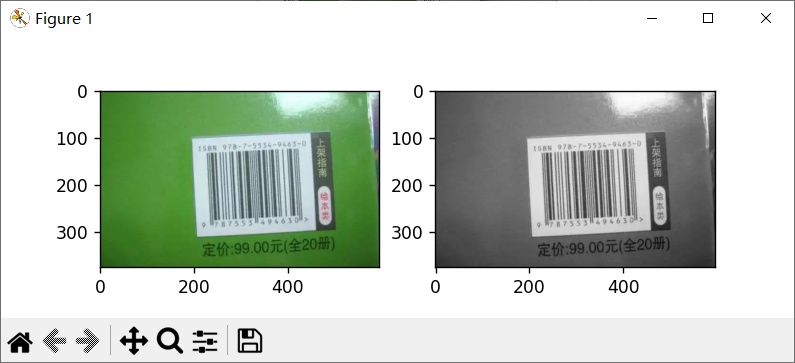
\includegraphics[height=120pt]{sample_toGrey}
    \caption{灰度化效果展示}
\end{figure}


\subsection{二值化}
根据课件(第9章-3基于阈值的图像分割)内容可知,可以按照图像的灰度不同,选取一个阈值 $x$,将灰度 $\ge x$ 的都转为一种灰度,其余的转为另一种灰度,实现二值化。

这个阈值如果手动选取的话适应性不够强,但是如果使用自适应阈值,即通过某种算法计算直接得到阈值 $x$,如 Otsu 算法,在实践验证中,发现效果也不是很理想。\textit{(Otsu 算法见下文算法比较)}

考虑采用一种比较朴素的思路,即枚举阈值。因为阈值的取值范围是 $[0,255]$。不妨以 $10$ 为公差,等差地枚举这个范围内的若干个阈值,然后以该阈值进行二值化。枚举次数约为 $25$ 次。显然,这么做的代价是,本来只需要对原图进行 $1$ 次识别 ISBN,会变成需要对原图进行至多 $25$ 次识别。不过,考虑到计算机算力较高,也能在相对可以接受的时间内求出结果。

为了提高效率,下面代码使用了矩阵运算加速。

二值化核心代码如下:
\begin{lstlisting}[language=python]
def toBinary(img, x, ltx=0, gex=255):
    '''传入灰度图img和阈值x,将其二值化并返回\n
    规定<x的染成白色(ltx),>=x的染成黑色(gex)'''
    img2 = img.copy()
    img2[img2 < x] = ltx
    img2[img2 >= x] = gex
    return img2
\end{lstlisting}

任取阈值(这里取的是 Otsu 算法求的阈值),运行效果如下:
\begin{figure}[htbp]
    \centering
    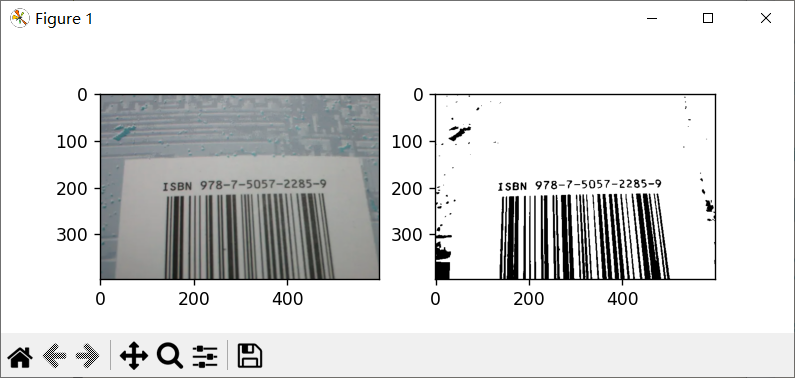
\includegraphics[height=120pt]{sample_toBinary}
    \caption{二值化效果展示}
\end{figure}

\begin{comment}
所以考虑用基本自适应阈值。采用 Otsu 算法(最大类间方差法),具体步骤如下:
设图像长宽为 $n,m$,最佳阈值是 $x$,$< x$ 的点有 $n_0$ 个,$\ge x$ 的点有 $n_1$ 个,原图 $< x$ 的点平均灰度为 $\mu_0$,$\ge x$ 的点平均灰度为 $\mu_1$,令:
\[w_0=\frac{n_0}{nm},\quad w_1=\frac{n_1}{nm}\]
显然满足:
\[n_0+n_1=nm,\quad w_0+w_1=1\]
则二值化前的均值 $\mu$ 显然满足:
\[\mu=w_0\cdot\mu_0+w_1\cdot\mu_1\]
为了让方差最大化,设方差 $\sigma$ 为:
\[\sigma=w_0\cdot(\mu_0-\mu)^2+w_1\cdot(\mu_1-\mu)^2\]

联立解得:$\sigma=w_0\cdot w_1\cdot (\mu_0-\mu_1)^2$,因此,将所有 $\ge x$ 的点与 $< x$ 的点分别染色为两种灰度,即可实现灰度化。

具体到代码实现上,可以枚举 $x\in[0,255]$,然后分别计算 $\sigma$,将取得最大 $\sigma$ 的 $x$ 作为阈值即可。

考虑到在本题中,一般是从按的背景上分割出暗的物体(即数字),所以将 $< x$ 的都染为黑色,$\ge x$ 的都染成白色。

上述代码涉及大量遍历图像的操作,将其用\textbf{矩阵运算优化},能显著提升运算效率。时间复杂度为 $O(255nm)$,对较小的图像能以几乎一瞬间求出结果。

核心代码如下:
\begin{lstlisting}[language=python]
import numpy as np
def getThrestHold(img):
    n, m = img.shape
    mx, x = -1, 0  # mx是当前最大值,x是取得最值的阈值
    np.seterr(divide='ignore',invalid='ignore')#零除
    for i in range(0, 256):
        n0 = np.sum(img < i)
        n1 = n*m-n0
        w0 = n0/(n*m)
        w1 = 1-w0
        mu0 = np.sum(img[img < i])/n0
        mu1 = np.sum(img[img >= i])/n1
        g = w0*w1*(mu0-mu1)**2
        if g > mx:
            mx, x = g, i
    return x
def toBinary(img, x, ltx=0, gex=255):
    img2 = img.copy()
    img2[img2 < x] = ltx
    img2[img2 >= x] = gex
    return img2
\end{lstlisting}
运行效果如下:
\begin{figure}[htbp]
    \centering
    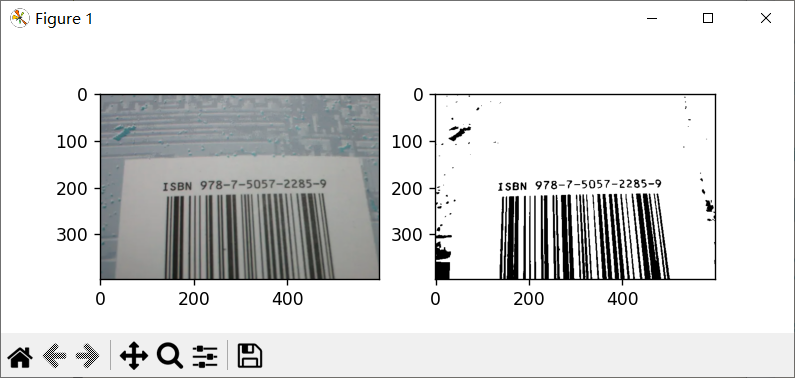
\includegraphics[height=120pt]{sample_toBinary}
    \caption{二值化效果展示}
\end{figure}
\end{comment}


\subsection{字符定位及分割}
基本原理:将图片二值化之后(假设背景是白色,其余是黑色),在理想情况下(没有旋转、没有多余内容、噪声等),如果统计每一行每一列有多少个黑点,绘制水平和垂直统计图。核心代码如下:
\begin{lstlisting}[language=python]
def getHoriAndVertSum(img):
    img1 = ((255-img)//255).astype(np.uint16)
    sumVert = img1.sum(axis=0)
    sumHori = img1.sum(axis=1)
    return [sumHori, sumVert]
\end{lstlisting}
可以发现ISBN的部分会呈现出一段特殊波的形状,如图所示:\textit{(作图代码见附录)}
\begin{figure}[H]%让插入的图片紧跟在文字后面
    \centering
    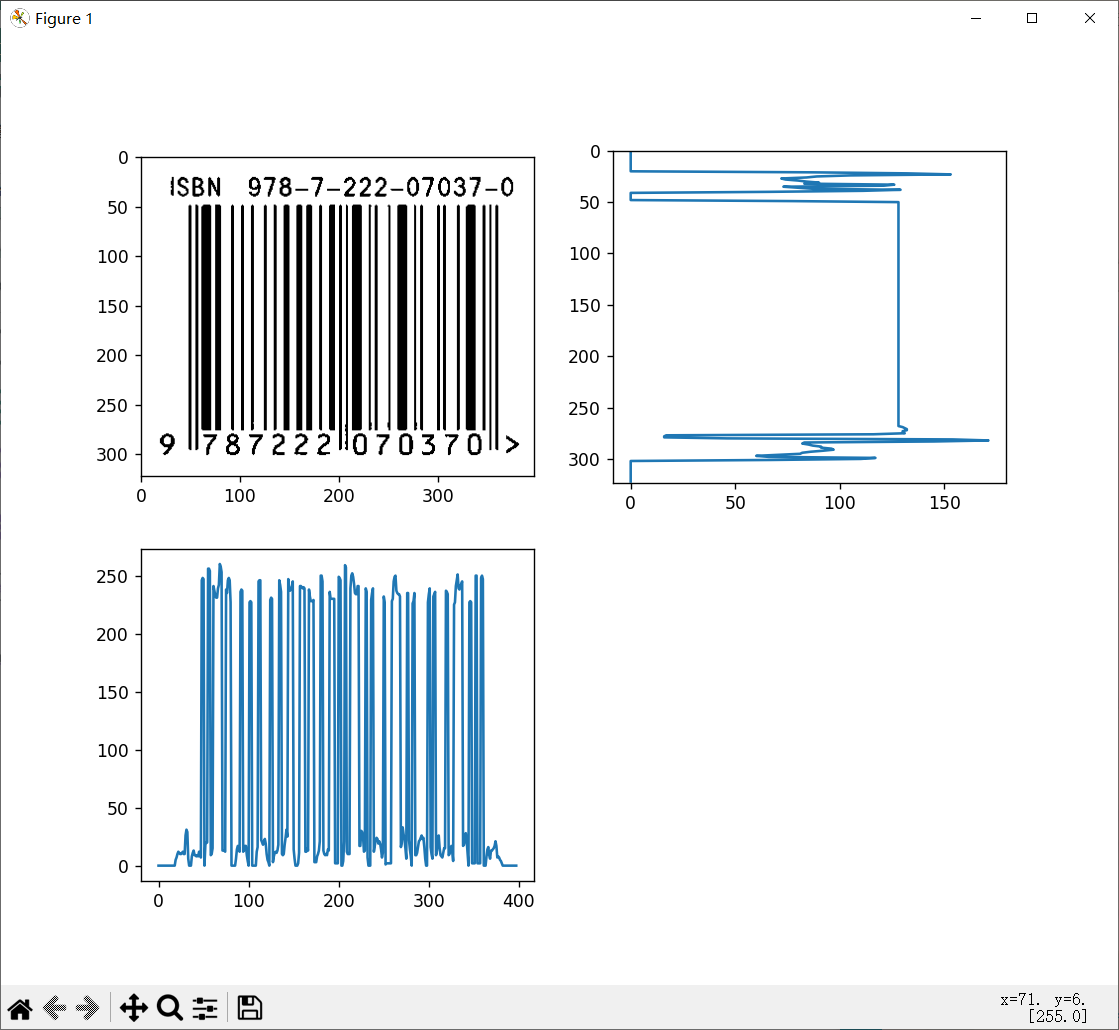
\includegraphics[height=260pt]{isbn_sum}
    \caption{ISBN图的统计特征}
\end{figure}

观察图像可知,垂直统计图的条形码处的波形波动也跟条形码一样剧烈变化,且水平统计图的条形码处是一段平的较高的图形。而ISBN号一定出现在其条形码的上下两端出现。根据ISBN号的知识可知,上下出现的数字通常是相同的\textit{(如果不同,一般一个是旧版ISBN,一个是新版ISBN,二者指向同一本书)}。则任取一边进行识别即可。

\textit{注:初始版本的实现采用的是有所不同的思路,后来实践效果很差故进行了改进优化,初始算法见下文算法比较。}

根据实践和调试经验,我们发现下面行与条形码距离太近,而且受到首尾条形码的干扰,较难识别。上面行间距大,干扰相对少。所以我们优先考虑识别上面的行,如果无法识别再考虑识别下面的行。

找到上述的每个波形,可以设置一个阈值 $low$,然后对离散函数 $f$(即每行/列下标为自变量,该行/列的黑点数为因变量的函数) 进行切割。作一条 $y=low$ 直线截断函数 $f$,所有函数值都 $\ge low$ 的区间值组成一个个波形,将这些区间记录下来即可。我们可以采用遍历的方法实现该操作,获取每个区间。

这个阈值 $low$ 的选取需要根据不同图像而做改变。不妨设 $f$ 的均值为 $\overline{f}$,设置 $low=0.32\overline{f}$。 

显然,数字行区间出现在条形码区间的上下。且条形码区间的长度是最长的。我们不妨先找到长度最长的区间,然后取其相邻的区间即可。

核心代码如下:
\begin{lstlisting}[language=python]
def getRanges(sums, low=0.32):
    '''输入向量,返回所有值>=low*均值的连续峰段'''
    lim = low*sums.mean()
    ans = []  # 所有函数值>=lim的区间端点[l,r]
    inLow = True  # 当前是否扫描到<lim的下标
    left, right = -1, -1  # 临时变量
    n = sums.shape[0]  # 总长
    for i in range(n):
        # 进入符合条件的区间
        if sums[i] >= lim and inLow:
            left, inLow = i, False
        # 退出符合条件的区间
        if sums[i] < lim and not inLow:
            right, inLow = i, True
            ans.append([left, right])
    return ans
def getNumberLineRange(sums, low=0.35):
    '''输入向量,返回一个数字行的下标范围[l,r]'''
    low = sums.mean()*low
    rng = getRanges(sums)
    if len(rng) == 0:  # 图片有误
        return [0, 0]
    # 找到最长的段对应的下标
    strip = max(rng, key=lambda x: x[1]-x[0])
    sid = rng.index(strip)
    if sid > 0:  # 上一段
        return rng[sid-1]
    if sid+1 < len(rng):  # 下一段
        return rng[sid+1]
    return [0, 0]  # 只有条形码
\end{lstlisting}

分割效果如下:
\begin{figure}[H]
    \centering
    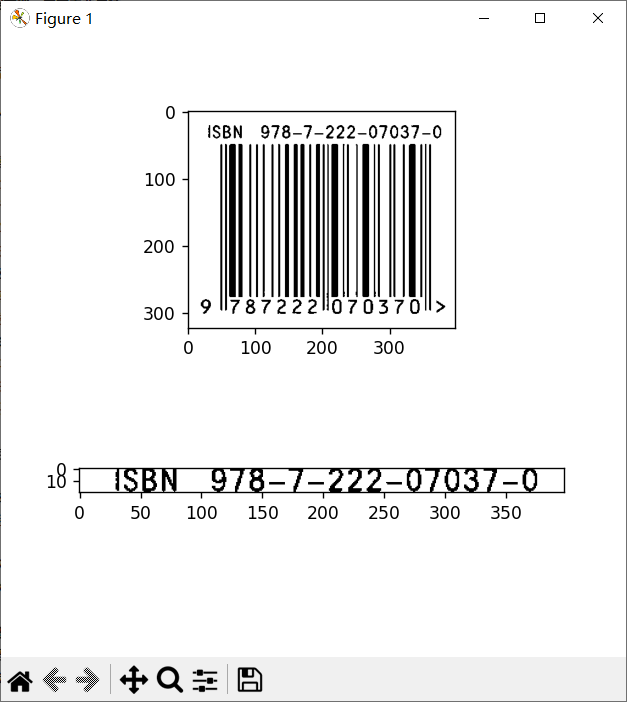
\includegraphics[height=120pt]{sample_splitRow2}
    \caption{按行分割效果}
\end{figure}

将其按行分割后,再次求其列特征,调用上述函数,得到统计图如下:
\begin{figure}[H]
    \centering
    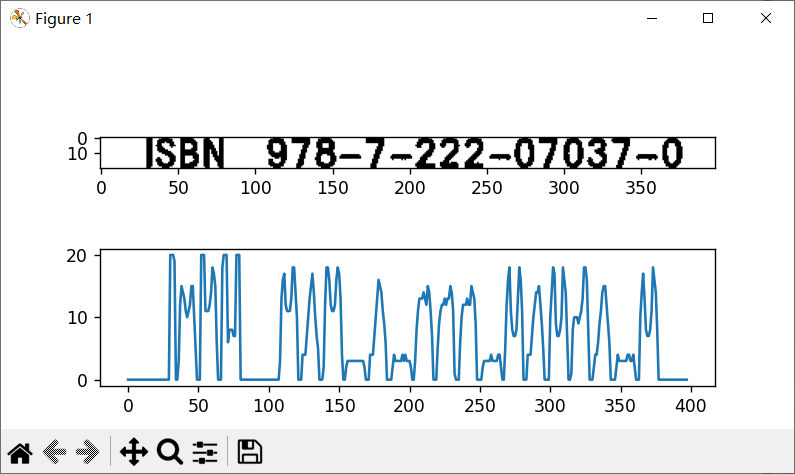
\includegraphics[height=120pt]{sample_splitRow_ana2}
    \caption{按行分割后的按行统计图}
\end{figure}

可以发现,每个字符都对应一段连续的波。按照类似上面的办法将其分割即可。直接调整上述代码\textit{(见附录)},得到效果如下:
\begin{figure}[H]
    \centering
    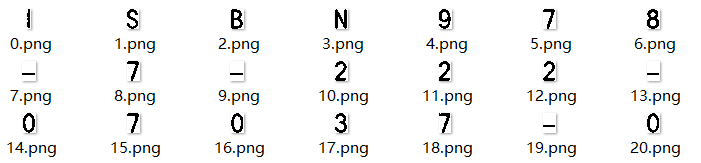
\includegraphics[height=80pt]{sample_splitNum2}
    \caption{分割后得到的每个字符}
\end{figure}

可以发现,分割出来的内容里含有无关的元素,包括 ISBN 四个字符和短横线 -。对复杂的图像,可能还有一些噪声、误点等。考虑如何初步筛除这些内容。

关于图像去噪,可以用滤波器等方法先做预处理。对短横线,不难发现其统计特征是,该字符只有少数行有黑点,大部分行没有黑点,不妨直接将大部分行基本是空白的字符给去除,这样可以把短横线和一些误点去除。还可能有一些大面积污点,其特征是几乎整个区域都是黑点,我们可以把这样的也去除。对 ISBN 四个字符,考虑在后续模板匹配时去除。

核心代码如下:
\begin{lstlisting}[language=python]
def filtRanges(img, arr):
    '''输入区间,返回经过初步筛选后的有效区间'''
    res = []
    h = img.shape[0]
    for l, r in arr:
        sub = img[:, l:r+1]
        blacks = sub[sub == 0].size
        lens = r-l+1
        tot = h*lens
        if blacks >= tot*0.7:  # 黑色太多
            continue
        sumH, sumV = getHoriAndVertSum(sub)
        vrows = sumH[sumH > 0.05*h].size
        if vrows < 0.28*h:  # 空白行太多
            continue
        res.append([l, r])
    return res
\end{lstlisting}

效果如下,去除横线的效果显著:
\begin{figure}[H]
    \centering
    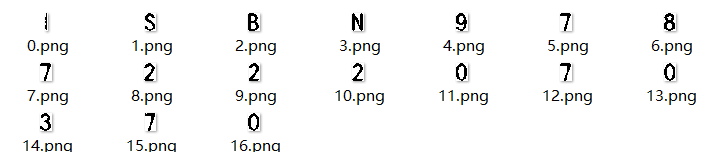
\includegraphics[height=70pt]{sample_splitNum_flit2}
    \caption{分割后得到的每个字符(经初步筛查)}
\end{figure}

将本节代码全部整合为一个函数,如下所示:
\begin{lstlisting}[language=python]
def splitNumbers(img):
    '''输入一张二值化图像
    返回其分割出来的字符子图列表'''
    sumHori, sumVert = getHoriAndVertSum(img)
    l, r = getNumberLineRange(sumHori)
    img2 = img[l:r, :]
    sumH2, sumVert2 = getHoriAndVertSum(img2)
    rng = filtRanges(
        img2, getRanges(sumVert2, 0.12))
    imgs = splitByVerts(img2, rng)
    return imgs
\end{lstlisting}

\subsection{预处理旋转}
上述字符定位与分割过程对理想状态的 ISBN 字符分割表现良好,但是并非所有图像都是理想的。最常见的就是存在旋转,如:

\begin{figure}[H]
    \centering
    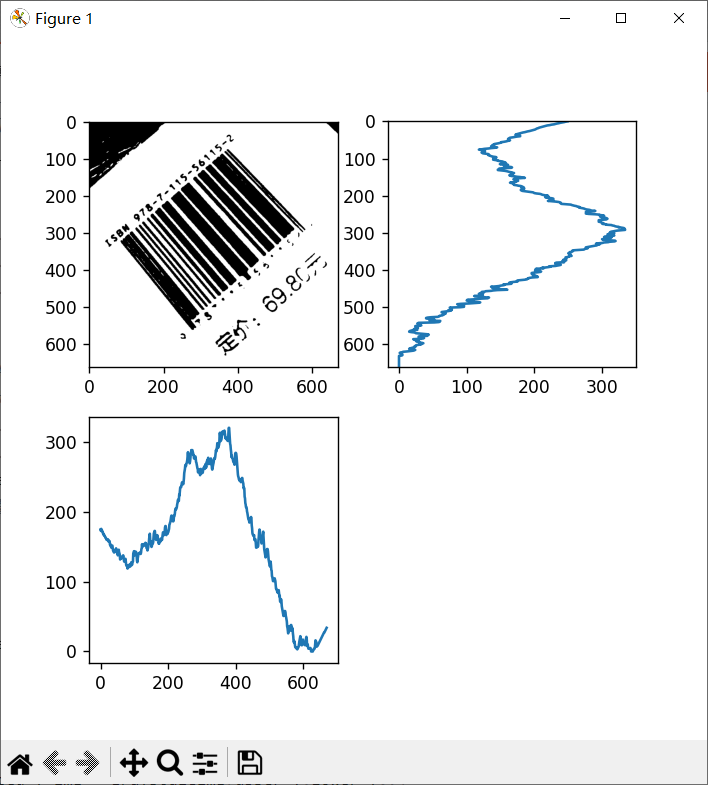
\includegraphics[height=260pt]{isbn_rotated}
    \caption{旋转过的ISBN图像及其分析}
\end{figure}

观察可知,ISBN 条形码明显的特征是有许多直线的条形,被旋转后,直线的朝向也会发生改变。如果我们能找出这些条形码直线及其旋转角,就能将其旋转回去。

根据课件(第9章-基于边缘检测的图像分割-Hough变换)可知,使用 Hough(霍夫)变换能够找到图中的直线。我们可以先使用 Canny 算子进行边缘检测,然后使用 Hough 变换对边缘检测结果提取其中的直线。

在实践过程中,不难发现,使用 Hough 变换需要设定一个阈值 $lim$,只有直线上的点数(即直线长度)超过 $lim$ 的直线才能被检测到。然而,图像变化多样,我们很难实现设定固定的 $lim$ 来满足不同的真实情境。因此,我采用了\textbf{倍增法}来快速枚举 $lim$ 的值,具体思想为:先设定一个较高的初始 $lim$,然后进行 Hough 变换找直线,如果找到的直线数目没有或很少,就证明阈值过高,这时将阈值除以一个常数来缩小阈值 $lim$,并继续查找,一直重复如上步骤直到找到为止。可以证明当阈值趋于 $0$ 时必然能找到。该算法能在对数复杂度内找到一个较为合适的阈值并进行直线分割。

核心代码如下:

\begin{lstlisting}[language=python]
def getLines(img):
    #传入二值化图像,输出其倍增法所有检测出来的直线
    #50,150是最小最大阈值,3是sobel卷积核大小
    edges = cv2.Canny(img, 50, 150, apertureSize=3)
    lim = int(np.min(img.shape)*0.8)
    while True:
        lines=cv2.HoughLines(edges,1,np.pi/180,lim)
        if type(lines) == type(None) 
            or len(lines) <= 5:
            lim = int(lim*0.9)
            continue#找不到/太少就不断缩小要求
        return lines
\end{lstlisting}

效果如图所示:

\begin{figure}[H]
    \centering
    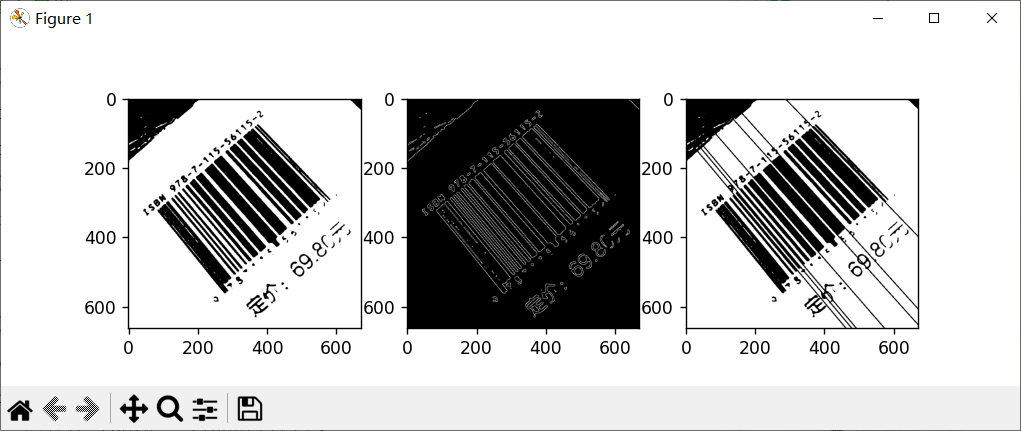
\includegraphics[height=120pt]{hough}
    \caption{Hough变换处理旋转图像提取直线并标注}
\end{figure}

进行上述过程后,实际上我们将得到一组直线。由于检测出来的直线不保证都是条形码上的直线,所以我们考虑选择这些直线里斜率处于中位数的作为图像的倾斜角,并对图像进行旋转还原。

Hough 变换得到的每条直线都是极坐标系下的 $(\rho,\theta)$ 参数,通过极坐标变换,可以计算出该直线在平面直角坐标下的任意两点,从而计算出直线的斜率。然后将直线斜率旋转到与纵坐标轴垂直即可。

代码如下:
\begin{lstlisting}[language=python]
def getMidAngle(lines):
    '''给定极坐标直线组,返回位于中位数斜角(角度制)'''
    lt = []
    for line in lines:
        rho, theta = line[0]
        a = np.cos(theta)
        b = np.sin(theta)
        x0 = a * rho
        y0 = b * rho
        x1 = int(x0 + 1000 * (-b))
        y1 = int(y0 + 1000 * (a))
        x2 = int(x0 - 1000 * (-b))
        y2 = int(y0 - 1000 * (a))
        k = np.arctan2(x2-x1, y2-y1)
        lt.append(k/np.pi*180)
    lt.sort()
    return lt[lines.shape[0]//2]
\end{lstlisting}

旋转时会产生新的图像区域,如果图片(书封面)本身是深色背景的,则图片边缘都是黑色的,应当用黑色填充;否则,应当用白色填充,可以进行特判,取出现频率最高的颜色进行填充。

进行旋转的核心代码如下:
\begin{lstlisting}[language=python]
def rotateImg(img, ang):
    #以中心旋转图像,顺时针转动ang角度并返回(白色填充)
    h, w = img.shape
    cx, cy = w//2, h//2
    # 1.0表示不缩放
    m = cv2.getRotationMatrix2D((cx, cy), -ang, 1.0)
    mc, ms = np.abs(m[0, 0:2])
    nw = int(h*ms+w*mc)
    nh = int(h*mc+w*ms)
    m[0, 2] += (nw/2)-cx
    m[1, 2] += (nh/2)-cy
    #分类讨论填充新区域的颜色
    numBlack = img[img == 0].size
    numWhite = img.size-numBlack
    if numBlack > numWhite:
        c = (0, 0, 0)
    else:
        c = (255, 255, 255)
    return cv2.warpAffine(img, m, (nw, nh),
            borderValue=c)
\end{lstlisting}

合并代码如下:
\begin{lstlisting}[language=python]
def autoRotate(img):
    '''以二值化图像为输入,输出自动旋转后的图像'''
    lines = getLines(img)
    ang = getMidAngle(lines)
    return rotateImg(img, ang)
\end{lstlisting}

效果图展示:
\begin{figure}[H]
    \centering
    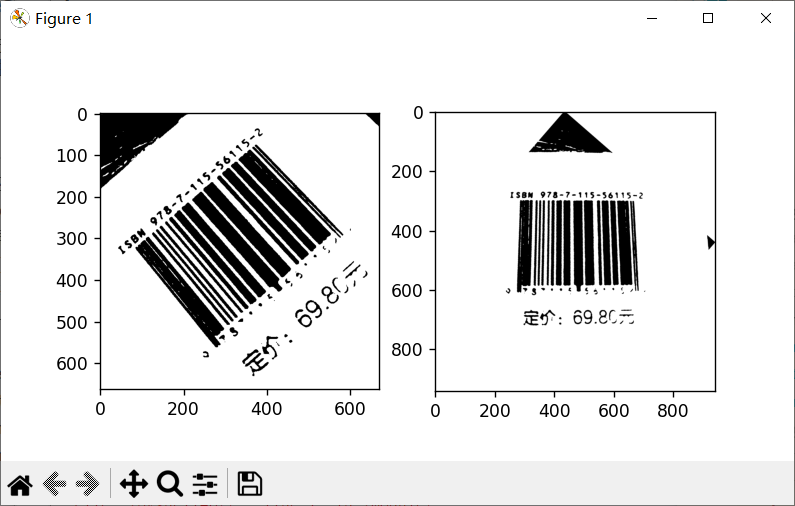
\includegraphics[height=120pt]{sample_autoRotate}
    \caption{将条形码自动旋转到垂直效果}
\end{figure}

显然,根据算法步骤可知,我们可以将条形码从“打横”的变成“打竖”的,但是旋转到大致垂直后,条形码上的字究竟是正的,还是反的,这是 Hough 变换无法实现的。为了解决这个问题,我们将在后续处理中,将图片分别当成是正的和反的都处理一遍,哪个匹配出更多内容就取哪个。

\subsection{预处理图片分割}
进行过预处理旋转后,仍有一个问题,如果图像不只有条形码,还有书本封面的其他内容,会干扰条形码的分析。所以我们希望能先预处理,使其只截取出条形码部分(如图3所示效果)。否则,其统计特征如下,进行分析困难:
\begin{figure}[H]
    \centering
    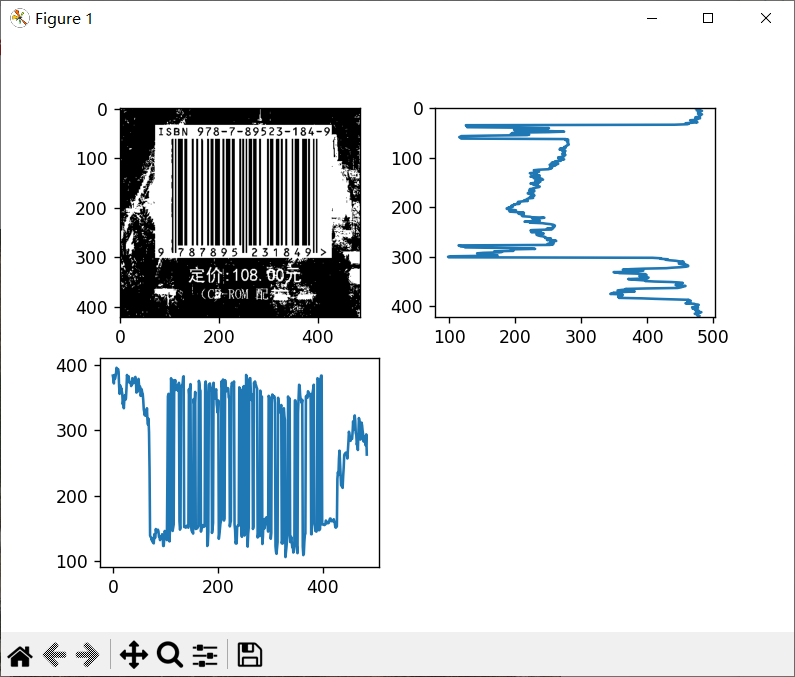
\includegraphics[height=120pt]{isbn_beforeCut}
    \caption{条形码外的封面内容干扰统计}
\end{figure}

\begin{comment}
根据课件(第12章-形态学图像处理)可知,数学形态学图像处理的基本思想是:用具有一定形态的结构元素(如一定大小的矩形、圆或菱形等)探测目标图像,能达到图像分析与识别的目的。因此,考虑使用形态学方法进行处理并提取出有效的子图区域。

观察可知,ISBN 的有效区域总是一个白色的矩形为背景的。我们可以考虑找到这个矩形区域并将其提取出来。

根据课件内容可知,闭运算(先膨胀再腐蚀)能磨光物体内边界,开运算(先腐蚀再膨胀)能磨光图像外边界。

根据类似的经验,我们可以先膨胀图像,将条形码矩形的内部内容去掉,用背景色替代,再进行一次腐蚀去噪。

不妨定义一个横向的长条矩形,如 $(n\times 1)$ 矩形进行膨胀;然后用 $(1\times m)$ 的纵向矩形进行腐蚀,去掉纵向的残留条形码等内容。考虑到膨胀与腐蚀操作的本质,我们认为 $n,m$ 的选取可以与具体图片的大小无关。这里使用的并非闭运算,因为前后不是同一个结构元素。根据经验,不妨设 $n=20,m=15$,实践表明,能取得较优的效果。

代码如下:
\end{comment}

检测一张图像中出现的矩形区域,可以采用 Suzuki, S. and Abe, K. 在论文(\textit{见参考文献})中提出的算法。调用相关算法后,我们能够得到图像上的所有轮廓。根据本题的特殊性,我们只需要选取其中的所有矩形轮廓。特别地,有时候如果轮廓检测失败,可能会得到许多很小的轮廓,不妨设置一个阈值如 $20\%$,所有面积小于原图像的 $20\%$ 的矩形全部忽略掉。然后,我们取出最大的矩形,作为检测的目标。

为了得到更准确的结果,我们需要实现进行预处理,例如可以先进行高斯模糊,然后再用 Canny 算法做边缘检测,以边缘检测结果的二值化图像开始提取轮廓。

核心代码如下:

\begin{lstlisting}[language=python]
def getMainRectangle(img):
    '''传入任意图像,返回其出现的最大矩形区域'''
    imgGray = toGrey(img)
    # 高斯模糊
    imgBlur = cv2.GaussianBlur(imgGray, (5, 5), 1)
    # Canny算子边缘检测
    imgCanny = cv2.Canny(imgBlur, 60, 60)
    # 边缘检测,RETR_TREE可能更精准
    contours, _ = cv2.findContours(
    imgCanny, cv2.RETR_TREE, cv2.CHAIN_APPROX_NONE)
    res = []  # 答案
    nh, nw = img.shape[:2]
    totArea = nh*nw
    for obj in contours:
        # 计算轮廓内区域的面积
        area = cv2.contourArea(obj)
        if area <= 0.2*totArea:  # 矩形太小
            continue
        # 计算轮廓周长
        perimeter = cv2.arcLength(obj, True)
        # 获取轮廓角点坐标
        approx = cv2.approxPolyDP(
            obj, 0.02*perimeter, True)
        CornerNum = len(approx)  # 轮廓角点的数量
        # 获取坐标值和宽度、高度
        x, y, w, h = cv2.boundingRect(approx)
        if CornerNum == 4:  # 是矩形
            res.append([x, y, w, h])
    if len(res) == 0:  # 找不到
        return [0, 0, nw, nh]
    # 取出最大的矩形
    ans = max(res, key=lambda x: x[2]*x[3])  
    return ans
\end{lstlisting}

效果如图所示:

\begin{figure}[H]
    \centering
    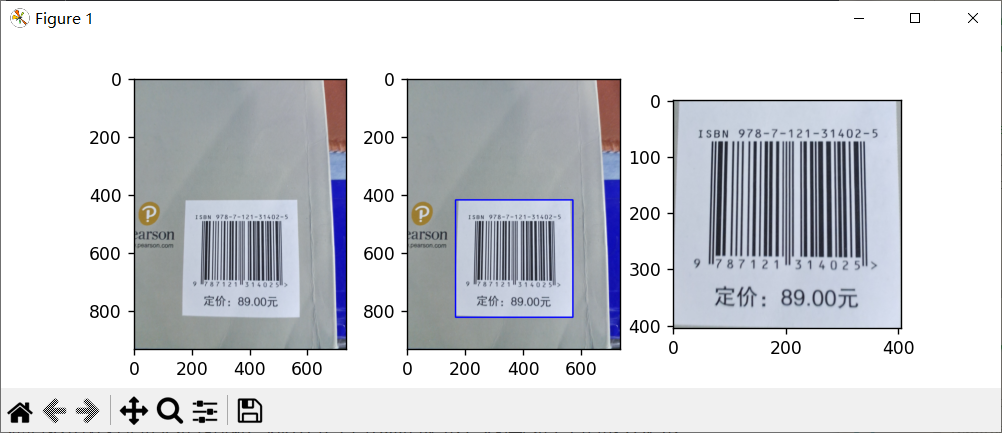
\includegraphics[height=120pt]{sample_graphSplit}
    \caption{截取图片中的矩形}
\end{figure}

然而,根据实践经验,直接进行矩形探测会有如下问题:如果书籍封面太花,即图案等干扰因素较多(如本节第一张图片)。为了达到更好的效果,我们可以进行两次分割。第一次分割直接调用上述做法,对第一次分割后的图像,再进行灰度化、二值化后进行第二次分割,以期望达到更好的效果。

如图所示(中图为第一次分割(找不到矩形),右图为第二次分割):

\begin{figure}[H]
    \centering
    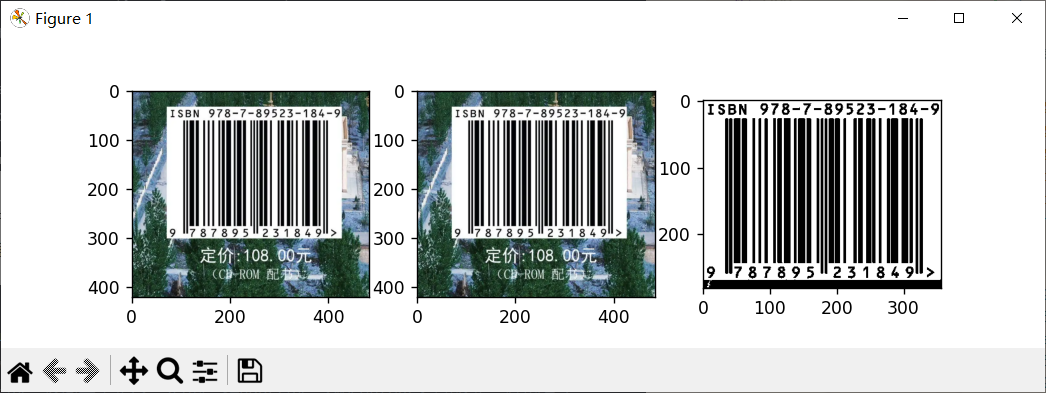
\includegraphics[height=120pt]{sample_graphSplit2}
    \caption{两次探测截取图片中的矩形}
\end{figure}


\subsection{字符识别}

因为上文我们已经分割出了每个字符,所以我们只需要对每个字符分别与每个标准字符进行比较,看其与哪个字符相似度最高,就认为它是哪个字符。

为了提高准确率,识别出不同的字体,我们考虑准备多套标准字符。经过对条形码的相关知识研究,我们发现 ISBN 条形码上主流的常见字体有两套,我们只截取与 ISBN 码相关的字符,如下图所示:

\begin{figure}[H]
    \centering
    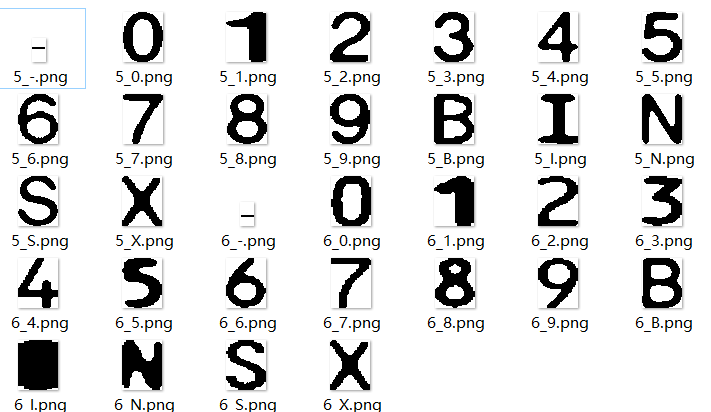
\includegraphics[height=120pt]{standard_fonts2}
    \caption{条形码字体的字符模板}
\end{figure}

接下来,对要识别的图片中分割出的每个字符,分别与每个标准模板进行比较,哪个相似度最高就认为该字符是哪个字符。在识别之前需要将待检测字符的图片长宽调整到与要比较的模板一致,进行大小归一化。

因为需要进行缩放,且上文分割出来的字符子图都是边缘几乎没有空白的。因此,如果模板的边缘较多空白,会在模板匹配时将字符子图拉长或压扁,从而使得匹配效果很差。因此,处理标准模板时,应当尽可能少留多余的空白区域,且保持正确的比例。

模板匹配是一种最原始、最基本的模式识别方法,研究某一特定对象物的图案位于图像的什么地方,进而识别对象物,这就是一个匹配问题。

模板匹配的主要原理为用如下公式计算相似性。设 $T(m,n)$ 是模板,$S(m,n)$ 是被搜索图。当两张图大小调整到相同时,相似性 $D$ 为:
\[D=\sum_{i=1}^m\sum_{j=1}^n(S(i,j)-T(i,j))^2\]

将其归一化,即相关系数 $R$ 为:

\[
R=\frac
{\sum_{i=1}^m\sum_{j=1}^nS(i,j)T(i,j)}
{\sqrt{\sum_{i=1}^m\sum_{j=1}^nS(i,j)^2}
\sqrt{\sum_{i=1}^m\sum_{j=1}^nS(i,j)^2}}
\]

使用如下公式,$R$的取值归一化到了 $[-1,1]$,且计算值越接近 $1$,表示越相关,越接近 $-1$ 表示越不相关。

根据公式可知,我们只需要对每个被搜索图,对每个模板都计算一次 $R$,计算得最大的那个字符就认为是结果。代码如下:

\begin{lstlisting}[language=python]
def compare(target, std):
    '''比较target与模板图像std的相似性并返回'''
    # 将target的大小缩放到与std一致
    target = cv2.resize(target, std.shape[::-1])
    res = cv2.matchTemplate(
        target, std, cv2.TM_CCOEFF_NORMED)
    # 返回值分别是min_val,max_val,min_loc,max_loc
    return cv2.minMaxLoc(res)[1]  # 只要maxval
def getNumber(src):
    '''将一张图片与全体模板比较
    取最大相似的字符作结果'''
    maxv, maxchar = 0, '?'
    for fi in range(2):  # fi是第几套字体
        for i in strname:  # i是字符值
            v = compare(src, tems[fi][i])
            if v > maxv:
                maxv, maxchar = v, i
    return maxchar
def getMatch(img):
    '''给定二值化图像,输出识别结果数组'''
    srcs = splitNumbers(img)
    return [getNumber(i) for i in srcs]
\end{lstlisting}

其中,上面代码的 tems 变量是一个列表,其元素是一个字典,字典元素是经过灰度化、二值化的从外部读入的模板图片。即相当于是一个模板的二维数组。

\subsection{ISBN号识别的优化调整}

下面展示优化匹配,提高准确率的修正算法过程。并在本节末提供整合本章全部小节的整合代码函数接口。

首先,匹配过程中会遇到 ISBN 四个字符,还可能会遇到未被初筛筛掉的短横线,我们需要在匹配结果中将其删掉。

经过实践表明,数字 0 与字符 B 具有较高的相似性,在匹配时可能会将 0 匹配为 B。然而我们知道,条形码行中只会出现最多一个 B,所以对匹配到的其他的 B,我们统统特判其视为 0。

因此,初步筛选的代码如下:
\begin{lstlisting}[language=python]
def filtRes(m):
    '''输入匹配结果,对结果进行筛除和修正'''
    r = []
    hasB = False  # 是否出现过B
    for i in m:
        # 首次出现B
        if i == 'B' and not hasB:
            hasB = True
            continue
        # 再次出现B,根据实践经验,结果应修改为0
        if i == 'B' and hasB:
            i = '0'
        # 只保留数字
        if i not in 'ISBN-':
            r.append(i)
    return r
\end{lstlisting}

之后,我们得到经过筛选的结果。由于在上文中,一来我们进行过旋转后无法判别正反,故对每张图片,我们将其分为原图和旋转 180 度后的图,分别需要进行判定。我们需要比较这两次识别,哪次是更优的,哪个就是正面作为结果,为此,我们首先需要判定怎样的结果是合理的。

根据相关知识,可知 ISBN 号有两种版本。不妨设第 $i$ 位 ISBN 号数字为 $m_i$。ISBN 号的最后一位是校验码 $s$,可以通过前面的数字位计算得知,如果计算结果与校验码一致,说明无误。

旧版 ISBN 号有十位,校验码计算公式为:
\[s=\sum_{i=1}^9m_i\cdot(11-i)\bmod{11}\]

如果 $s\le 9$,则校验码就是 $s$;否则 $s=10$,校验码为 X。

新版 ISBN 号有十三位,校验码计算公式为:
\[s=(10-(\sum_{i=1}^6m_{2i-1}+\sum_{i=1}^63m_{2i})\bmod 10)\bmod{10}\]

即奇数位权重 $1$,偶数位 $3$。$s$ 就是校验码。

特别地,在某些时候,有小概率 AI 会把大量的噪声或错误图像认定为数字,且存在全零序列满足上面的校验码规则,即无效 ISBN 码 $00\cdots 0$ 也被认为是正确的。

这时,根据统计规律,ISBN 码中每个数字出现的频率应该近似大致相等\textit{(事实上严格来说不是,因为 ISBN 码每一段有严格的格式编码要求)},所以不妨近似地认为 ISBN 码的平均数应该接近 $\frac{1}{10}\sum_{i=0}^9i=4.5$。如果我们比较的两方都满足校验码规则,则取更接近 $4.5$ 的一个作为合法 ISBN 码。

因为这个判断的代码冗长,故不列出具体实现,可在项目中具体查看。这里只给出伪代码。
\begin{algorithm}
    \caption{比较两个ISBN序列哪个更合法(betterMatch)}
    \label{betterMatch}
    \renewcommand{\algorithmicrequire}{\textbf{输入:}}
    \renewcommand{\algorithmicensure}{\textbf{输出:}}
    \begin{algorithmic}
        \REQUIRE ISBN号序列 $m_1,m_2$
        \ENSURE 更佳的序列 $m$
        \STATE 对 $m_1,m_2$ 进行初筛分别得到序列 $d_1,d_2$
        \STATE 求 $d_1,d_2$ 的 ISBN 校验码是否合法
        \IF{二者都合法}
        \STATE 求 $d_1,d_2$ 的平均数
        \RETURN 平均数较与 $4.5$ 更接近的一方
        \ELSE
            \IF{其中一个合法}
            \RETURN 合法的一方
            \ELSE
                \IF{有一方长度为 $13$ 或 $10$}
                \RETURN 优先任选长为 $13$ 的,其次选 $10$ 的
                \ELSE
                \RETURN 任选一个
                \ENDIF
            \ENDIF
        \ENDIF
    \end{algorithmic}
\end{algorithm}

经由上述算法,我们可以对一张设定了特定二值化阈值的图片进行比较,从而解决了上文的正反面问题:

\begin{lstlisting}[language=python]
def matchFlip(img):
    '''输出一张图片,将其正反都匹配一次取最优'''
    img1 = img.copy()
    img2 = rotateImg(img1, 180)
    res1 = getMatch(img1)
    res2 = getMatch(img2)
    return betterMatch(res1, res2)
\end{lstlisting}

最后,我们采取枚举二值化阈值的办法,调用上述算法,对多个结果分别比较,每次将计算出来的新结果与历史最优结果比较,然后取最优的结果作为 ISBN 号识别结果。

特别地,在一些时候,考虑到拍摄不全等原因,最右边界的数字经常会残缺。如果我们匹配出了正常长度,但是不满足校验码规则的结果,我们不妨用 ISBN 号校验码算法求出最后一位的值。即:

\begin{lstlisting}[language=python]
def adjudgeByChecksum(m):
    if len(m) not in (10, 13):
        return m  # 长度不对无解
    if m[:-1].count('X'):
        return m  # 非末位有X无解
    if not checkISBN(m): # 不合法就校正
        m[-1] = getChecksum(m)
    return m 
\end{lstlisting}

此外,手机拍摄的图片的像素值很大。而做识别无需用到这么大的像素,因为模板本身像素较低,比较时也会将图像缩放。所以,如果图片本身大小过大,不妨先等比例缩放一下,让其保持比较适合的尺寸,以提高计算速度。

调整尺寸的代码如下:

\begin{lstlisting}[language=python]
def reshape(img, mw=1000, mh=1000):
    '''给定图片,等比例裁剪使长宽不超mw,mh'''
    h, w = img.shape[:2]
    sh, sw = mh/h, mw/w
    s = min(sw, sh, 1)  # 与1比较,防止放大
    res = cv2.resize(img, (0, 0), fx=s, fy=s)
    return res
\end{lstlisting}

因此,对图片的预处理,包括自动旋转与旋转后自动调节大小,即:

\begin{lstlisting}[language=python]
def autoRotateC(img):
    '''以彩色图像为输入,输出自动旋转后的图像'''
    img2 = toGrey(img)
    img2 = toBinary(img2, getThrestHold(img2))
    lines = getLines(img2)
    ang = getMidAngle(lines)
    return rotateImg(img, ang)
def preDeal(img0):
    '''给定一张图片,将其裁剪大小和自动旋转'''
    img = autoRotateC(img0)
    img = reshape(img)
    return img
\end{lstlisting}

之后,根据上文描述,我们两次识别裁剪的方法将旋转后的图像裁切,使其只包含条形码部分:

\begin{lstlisting}[language=python]
def autoCut(img0, thr):
    '''传入彩色图像,两次匹配找到最大矩形区域子图\n
    返回结果是二值化后的子图'''
    img = cutImage(img0)
    img = toGrey(img)
    img = toBinary(img, thr)
    img = cutImage(img)
    return img
\end{lstlisting}

之后,进行字符匹配并做优化处理,得到最终结果并返回。本章的所有内容可以凝练为下面的函数接口:

\begin{lstlisting}[language=python]
def iterMatch(img0):
    '''给定一张图片,枚举二值化阈值取最好结果\n
    输出其ISBN字符串结果(以列表形式)'''
    img = preDeal(img0)
    ans = []  # 当前最优结果
    for thr in range(5, 255, 10):
        img1 = autoCut(img, thr)
        res = matchFlip(img1)
        print(thr, res)
        ans = betterMatch(ans, res)
    return adjudgeByChecksum(ans)
\end{lstlisting}

\begin{comment}
下面展示了截取的三种不同的字体下的数字0-9和其他符号的图像的标准图像,从上到下分别是方正舒体、宋体、清松手写体。如图所示:

\begin{figure}[H]
    \centering
    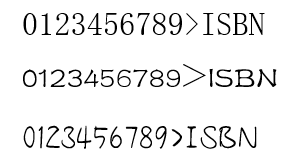
\includegraphics[height=120pt]{standard_fonts}
    \caption{标准字体}
\end{figure}

采用与上文字符分割一节类似的办法,对这三张图片预处理,得到每个数字。
\end{comment}

\section{实验结果及分析}
\subsection{不同算法比较}

\subsubsection{二值化}
在初版设计中,我采用了采用 Otsu 算法(最大类间方差法),具体步骤如下:

设图像长宽为 $n,m$,最佳阈值是 $x$,$< x$ 的点有 $n_0$ 个,$\ge x$ 的点有 $n_1$ 个,原图 $< x$ 的点平均灰度为 $\mu_0$,$\ge x$ 的点平均灰度为 $\mu_1$,令:
\[w_0=\frac{n_0}{nm},\quad w_1=\frac{n_1}{nm}\]
显然满足:
\[n_0+n_1=nm,\quad w_0+w_1=1\]
则二值化前的均值 $\mu$ 显然满足:
\[\mu=w_0\cdot\mu_0+w_1\cdot\mu_1\]
为了让方差最大化,设方差 $\sigma$ 为:
\[\sigma=w_0\cdot(\mu_0-\mu)^2+w_1\cdot(\mu_1-\mu)^2\]

联立解得:$\sigma=w_0\cdot w_1\cdot (\mu_0-\mu_1)^2$,因此,将所有 $\ge x$ 的点与 $< x$ 的点分别染色为两种灰度,即可实现灰度化。

具体到代码实现上,可以枚举 $x\in[0,255]$,然后分别计算 $\sigma$,将取得最大 $\sigma$ 的 $x$ 作为阈值即可。

考虑到在本题中,一般是从按的背景上分割出暗的物体(即数字),所以将 $< x$ 的都染为黑色,$\ge x$ 的都染成白色。

上述代码涉及大量遍历图像的操作,将其用矩阵运算优化,能显著提升运算效率。时间复杂度为 $O(255nm)$,对较小的图像能以几乎一瞬间求出结果。

核心代码如下:
\begin{lstlisting}[language=python]
import numpy as np
def getThrestHold(img):
    n, m = img.shape
    mx, x = -1, 0  # mx是当前最大值,x是取得最值的阈值
    np.seterr(divide='ignore',invalid='ignore')#零除
    for i in range(0, 256):
        n0 = np.sum(img < i)
        n1 = n*m-n0
        w0 = n0/(n*m)
        w1 = 1-w0
        mu0 = np.sum(img[img < i])/n0
        mu1 = np.sum(img[img >= i])/n1
        g = w0*w1*(mu0-mu1)**2
        if g > mx:
            mx, x = g, i
    return x
\end{lstlisting}

这种算法的理论是很好的,但是在实践中我们发现了如下问题:如果要识别的图片除了 ISBN 区域外,还有较大片的封面内容,那么这些封面内容有可能要么颜色过浅、要么颜色过剩,他们都会干扰方差,从而使得二值化效果很差,不利于后续的图片切割等处理。

基于这个缺陷,我们在上文中最终替换了算法,最终版本如上文所示。

\subsubsection{字符分割}
在初版设计中,我采用了如下的思路分割行:

数字区域的水平特征是,出现在条形码区域的附近,且边界是低频率的。那么我们可以先按水平特征截取出数字行,再进一步分析。在实现上,可以设一个低频阈值 $low$,如果某一行出现黑点个数 $\ge low$,就开始记为边界,直到下一次再出现 $< low$ 的行就设为另一边界,并把边界之间的行全部提取出来。根据肉眼观察和经验推理,不妨预设 $low=25\%max$,即最高频次的 $25\%$。

核心代码如下:
\begin{lstlisting}[language=python]
def getNumberLineRange(sumHori, low=0.25):
    lim = np.max(sumHori)*low  # 实际阈值
    left, right = -1, -1
    n = sumHori.shape[0]
    for i in range(n-1, -1, -1):
        if sumHori[i] >= lim and right == -1:
            right = i
        if sumHori[i] < lim and right != -1:
            left = i
            break
    return [max(0, left), max(0, right)]
\end{lstlisting}

该设计具有缺陷如下:

一、会被定价干扰。在ISBN里,定价附在矩形框内是很正常的,而且通常是在最下方。那么自底向上遍历,找到的行将会是定价这一行。(如测试集09)

二、无法解决残缺图像。如果拍照者只拍摄了上方的条形码,则自底向上找到的第一行是条形码。

三、基于最大值作阈值判断,稳定性不强。如果一张图片的边缘是全黑的,阈值会过高,导致判断失败。

四、虽然下面的数字行没有 ISBN 字符和横线,但是其与条形码过于接近,很容易被条形码干扰,特别是图片拍摄条件不良时,或者条形码与其间距太近时,又有轻微旋转干扰的话,可能很难分割出来。

基于这些缺陷,我们在上文中最终改进了算法。最终版本如上文所示。

\subsubsection{字符识别}
在初版设计中,我使用了方正舒体、宋体、清松手写体。如图所示:

\begin{figure}[H]
    \centering
    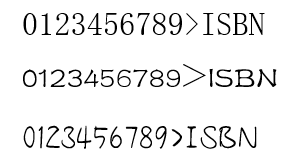
\includegraphics[height=90pt]{standard_fonts}
    \caption{标准字体}
\end{figure}

将其进行字符分割,得到标准模板。然而,其效果并不好,连最简单最规范的 ISBN 图片都无法识别。


\section{总结与体会}
\section{致谢}
\section{参考文献}

%没弄明白
% \begin{thebibliography}{99}
%     \bibitem[otsu] 1tsu 算法解析
% \end{thebibliography}

\textit{(注:红色的是超链接,点击可以跳转到原文。)}

\begin{enumerate}
    \item \href{https://blog.csdn.net/a15779627836/article/details/124151125}{Otsu 算法解析}
    \item \href{https://www.cnblogs.com/skyfsm/p/8029668.html}{数字分割}
    \item \href{https://blog.csdn.net/weixin_42272768/article/details/111244896}{Canny边缘检测}
    \item \href{https://blog.csdn.net/qq_30460949/article/details/90293147}{Hough变换详解1}
    \item \href{https://blog.csdn.net/qq_41112170/article/details/125729100}{Hough变换详解2}
    \item \href{https://blog.csdn.net/wyx100/article/details/80541726}{图片旋转}
    \item \href{https://blog.csdn.net/weixin_47365088/article/details/116566822}{提取特定图片区域}
    \item \href{https://blog.csdn.net/LPYchengxuyuan/article/details/122003702?utm_medium=distribute.pc_relevant.none-task-blog-2~default~baidujs_baidulandingword~default-0-122003702-blog-124125975.pc_relevant_aa&spm=1001.2101.3001.4242.1&utm_relevant_index=3}{形状识别}
    \item 边缘检测 Suzuki, S. and Abe, K., TopologicalStructural Analysis of Digitized Binary Images by Border Following.CVGIP 30 1, pp32-46 (1985)
    \item 数字图像处理基础课程的全部课件 梁艳老师
\end{enumerate}

\section{附录}

\end{document}